\documentclass[12pt]{article}
\usepackage[spanish]{babel}
\usepackage[utf8]{inputenc}
\usepackage[T1]{fontenc}
\usepackage{geometry}
\usepackage{fancyhdr}
\usepackage{graphicx}
\usepackage{float}
% Configuración de márgenes
\geometry{a4paper, left=2.5cm, right=2.5cm, top=3cm, bottom=3cm}

% Configuración de encabezado y pie de página
\pagestyle{fancy}
\fancyhf{}
\lhead{Proyecto 1 Sistemas Operativos}
\cfoot{\thepage}

\begin{document}

\title{Proyecto 1}
\author{Roberto Artigues, Emilio Meza, Nicolás Soto}
\date{8 de Octubre de 2023}
\maketitle


\section{Introducción}
Desarrollo de un intérprete de comandos simple en Linux (shell). La shell a implementar será similar
a las disponibles actualmente en Linux.
\section{Parte 1}

La Parte 1 del código se encarga de implementar una shell simple que cumple con los siguientes requisitos:

\begin{enumerate}
\item Proporciona un prompt (indicador de modo de espera de comandos) para que el usuario ingrese comandos.
\item Lee el comando ingresado por el usuario desde la entrada estándar y lo parsea para identificar el comando y sus argumentos, con la capacidad de manejar un número indeterminado de argumentos.
\item Ejecuta el comando ingresado en un proceso hijo utilizando las llamadas al sistema \texttt{fork()} y \texttt{exec()}. La shell espera a que el comando en ejecución termine antes de mostrar nuevamente el prompt.
\item Maneja la entrada en blanco (cuando el usuario presiona "enter") imprimiendo nuevamente el prompt.
\item Soporta comandos que se comunican mediante pipes (\texttt{|}), lo que permite redirigir la salida de un comando como entrada para otro comando.
\item Puede finalizarse si se ingresa el comando "\texttt{exit}".
\item Proporciona un mensaje de error si se ingresa un comando que no existe.
\end{enumerate}

La parte principal del código ejecuta un bucle infinito donde se espera que el usuario ingrese comandos. Luego, se parsea la entrada del usuario, se crean procesos hijos para ejecutar los comandos, y se maneja la comunicación a través de pipes. El código también verifica y ejecuta el comando \texttt{start\_daemon} con dos argumentos (t y p) para iniciar la Parte 2 del código.

\section{Parte 2}

La Parte 2 del código se encarga de crear un demonio que mide y registra información del sistema en el archivo de registro del sistema \texttt{/var/log/syslog}. Esta parte cumple con los siguientes requisitos:

\begin{enumerate}
\item Crea un demonio que recopila información del sistema cada $t$ segundos durante un tiempo total de $p$ segundos.
\item El demonio extrae información como "processes", "procs\_running" y "procs\_blocked" del archivo \texttt{/proc/stat} para sistemas Linux.
\item Utiliza llamadas al sistema como \texttt{fork}, \texttt{umask}, \texttt{setsid}, \texttt{openlog}, \texttt{syslog}, y \texttt{closelog} para configurar y gestionar el demonio.
\item Puede ser detenido mediante el comando \texttt{killall} de Linux.
\end{enumerate}

El código utiliza \texttt{fork} para crear un proceso hijo que se convierte en un demonio (daemon) utilizando \texttt{setsid}. Luego, el demonio recopila información del sistema a intervalos regulares y la registra en el archivo de registro del sistema usando las funciones de registro de \texttt{syslog}. El demonio se puede detener utilizando \texttt{killall}.
\begin{figure}[H]
    \centering
    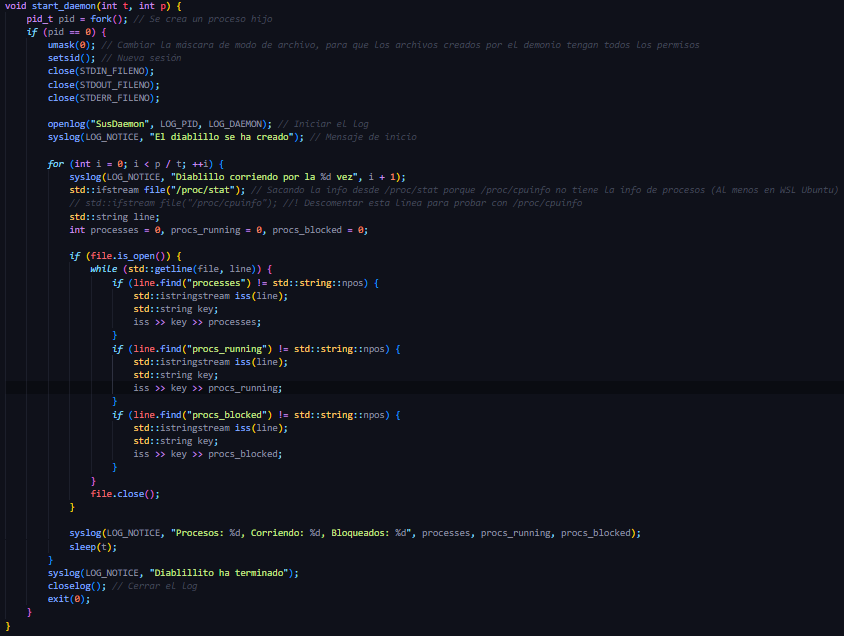
\includegraphics[width=0.7\textwidth]{daemon.png}
    \caption{Funcion Demonio}
\end{figure}
\begin{figure}[H]
    \centering
    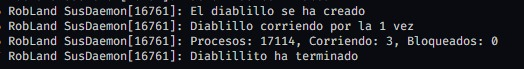
\includegraphics[width=0.7\textwidth]{demonio-working.jpeg}
    \caption{Demonio haciendo sus procesos}
\end{figure}

\end{document}